\section{Conceptual Framework}

This section provides an Input-Process-Output framework (IPO) as a basis for conceptual framework outlining the development and implementation of Shelter Location-Allocation System for Hagonoy, Bulacan. The IPO model was first introduced in the context of computer programming and documentation using the Hierarchy plus IPO (HIPO) technique. Moreover, the concept of input and output has been used before in economics, back in the 1930s, Wassily Leontief first conceptualized input-output analysis to illustrate economic interrelationships
 
 \begin{figure}[h!]
 	\centering
 	\caption{IPO Model} \label{fig:ipo}
 	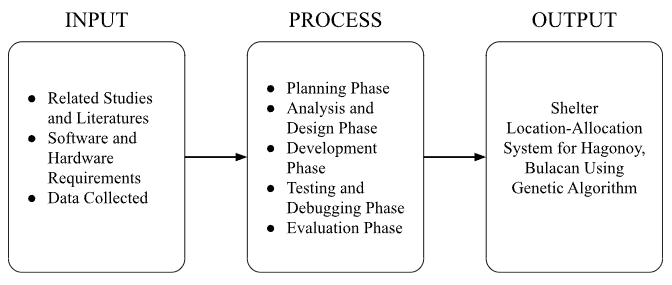
\includegraphics[width=\linewidth]{IPO}
 \end{figure}
 
The inputs for this project include related studies and literature, which provide a foundation for selecting and adapting an appropriate model for our system. These resources will be analyzed and synthesized to establish a strong foundation in conducting this project. We also need to gather software and hardware requirements, such as the compatible Windows version and system prerequisites, to ensure a smooth development process. Additionally, real data from Hagonoy, Bulacan, specifically community and shelter information, will be essential for testing and validating the system.

The process begins with planning, where we outline the objectives and approach for building the system. Once a clear plan is established, we proceed to analysis and design, which involves creating mock-up designs, an ERD schema, and process flows to help the developers visualize the system structure. The development phase is the longest phase, involving both frontend design and backend coding using the Qt framework. Once developed, the system undergoes rigorous testing to identify and correct any errors or anomalies, which will then be debugged or will be resolved. Finally, the system will be evaluated through a survey based on the ISO 25010 criteria to assess its acceptability.

The expected output is a fully functional decision support system that incorporates the  model adopted using a genetic algorithm as the solving method. The researchers will generate results showing the optimal shelter location-allocation for Hagonoy, Bulacan using the developed system.

 